\subsection{ALEXIS} 

Alexis and Maxime Jacque are working at the LF2L in the framework of "Introduction to the research" module.
The time is September 11 to October 11

\subsection{Context of their mision}

The context of the project is the extrusion process at LF2L (figure \ref{Context.Nicolas.Maxime})

\begin{figure}[H]
	\centering
	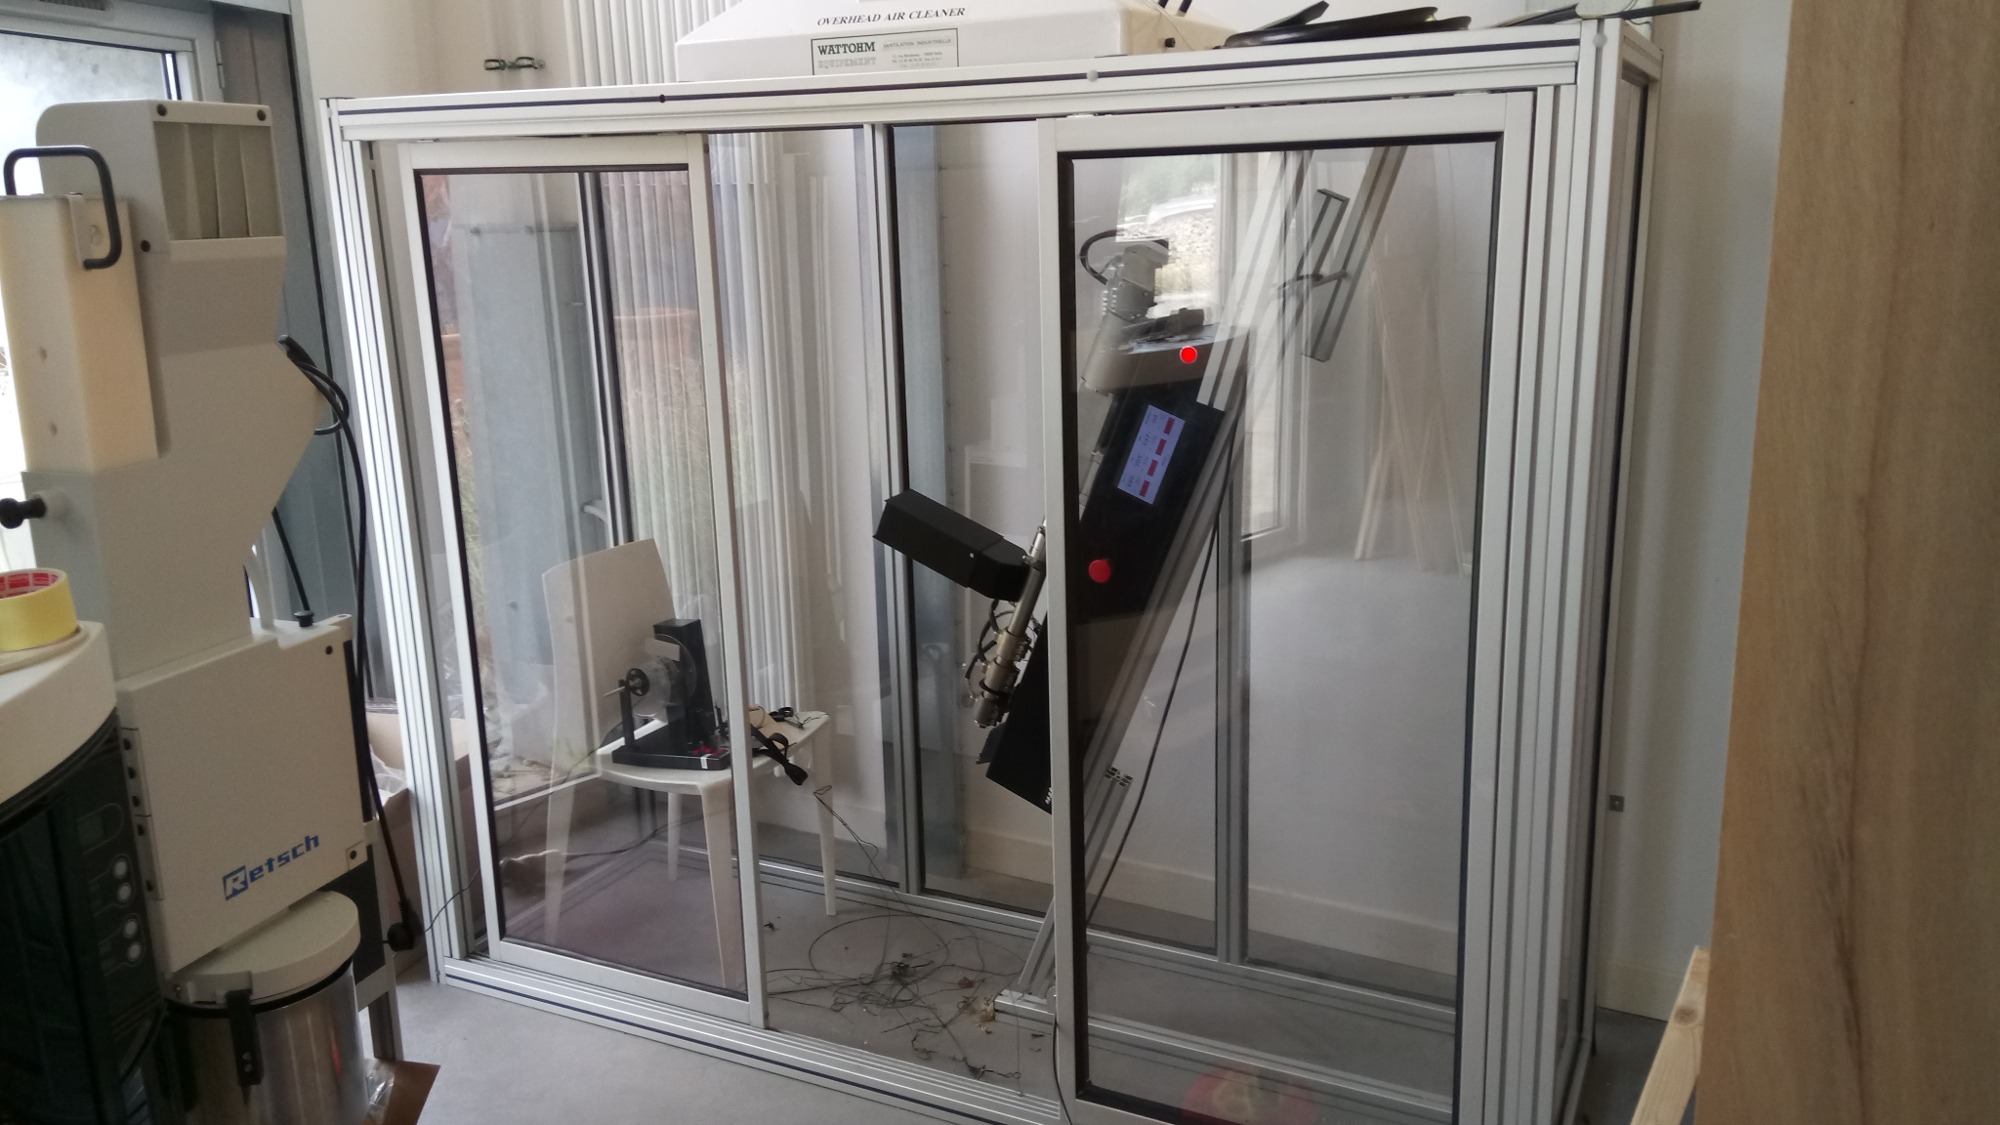
\includegraphics[width=0.7\textwidth]{Figures/Extrusion/Extruder.jpg}
	\caption{Extrusion process at Lorraine Fab Livin Lab}
	\label{Context.Nicolas.Maxime}
\end{figure}


\subsection{Objectives of the project}


The goal of the stage is to define and testing a functional prototype for feeding process in the extrusion machine at LF2L.




\begin{itemize}
	\item Exploration of concepts
	\item Definition of the operational conditions
\end{itemize}


Elements to consider:

\begin{itemize}
	\item State of the Art about Quality in 3D printing.
	\item Grey literature of 3D printing. 
\end{itemize}


\subsection{Expected elements to the end of the project}

The following elements are expected as results:

\begin{itemize}
	\item Tutorial to use the prototype
	\item Functional prototype
	\item Poster (Infography)  about the printing process at LF2L.
\end{itemize}

